\documentclass{article}
\usepackage{graphicx} % Required for inserting images
\usepackage[a4paper,left=2.5cm,right=2.5cm,top=2cm,bottom=2cm]{geometry}
\usepackage{minted}
\usepackage{lipsum} % Package for generating dummy text

\usepackage{mdframed}



\setminted{fontsize=\small, baselinestretch=1}


\title{%Decentralized Finance \\
  \large {Inoffical Course Script}
\author{Sarah Kuhn}
\date{April 2024}
}

\begin{document}
\maketitle
\thispagestyle{empty} % Remove page number from the first page

\newpage
\pagenumbering{arabic} % Start page numbering from 1
\setcounter{page}{1} % Set page counter to 1

\section{Finance Basics}
To begin we will first cover some fiance basics and underline why we need finical markets and what value they bring. Then we will discuss the key differences between CeFi and DeFi.
\subsection{Financial Markets: Underlying assumptions} 
Before we  talk about financial markets and their role in the economy, we first fix on what we base our analysis and reasoning about financial markets on. Obviously financial markets have a lot of real-life complexities and depend on decision from billions of individuals. Thus the assumption we make should provides a simplified framework that makes it easier for  to model complex financial systems. Economists often assume rational behavior and market efficiency, which then allows them to develop models and theories that help explain observed phenomena and make predictions seen in the markets.
\begin{itemize}
    \item \textbf{Rational Expectations}

Definition: Rational expectations describe that individuals make predictions about the future based on all available information and use these predictions to make decisions. These expectations are considered "rational" because they are consistent with the information available at the time.

In Financial Markets: Rational expectations imply that investors incorporate all available information, including past prices, economic data, and news, into their forecasts of future asset prices. This means that asset prices reflect the collective wisdom and expectations of investors, leading to efficient market outcomes. It also implies that actors won't make constant mistakes in predicting the future, which also means predicting the risks. 

    \item \textbf{Efficient Financial Market Theory}

    Definition: Efficient market theory suggests that financial markets quickly and accurately incorporate all available information into asset prices. So "asset prices represent the best possible estimates of the risk attached to them" (from lecture slide). Thus the risk from a financial market or just an investment can be inferred through mathematical analysis.

    \end{itemize}

\subsection{Role of Financial Markets} 
Financial markets play crucial role in our economy as they serve several purposes:
\begin{itemize}
    \item \textbf{Raising Capital}: Think of the financial market as a giant fundraising platform. It's where companies and governments go to ask investors for money. They can do this by selling parts of their company or borrowing money. This cash infusion helps them operate their businesses or kick start new projects.
    
    \item \textbf{Economic signaling}: We could also call this "setting fair prices": In the financial market, prices of assets like stocks and bonds are determined by how much people want to buy or sell them. This process helps investors know if they're paying a reasonable price for what they're investing in.
    \item \textbf{Ease of trading}: The financial market makes it convenient for people to buy and sell assets like stocks and bonds whenever they need to. This flexibility is crucial because it allows investors to adjust their portfolios swiftly in response to changing circumstances. We often say that a financial market provides liquidity to investors.
    \item \textbf{Risk management}: Within the financial market, there are tools available to help individuals protect their investments from unexpected events that could cause losses, like sudden market fluctuations or unexpected inflation. This is called " hedging against risk". Investors can protect themselves from adverse movements of factors that affect their value of assets. One can use
    instruments like options, futures or swaps to hedge against a potential decrease in a stock's value. In simple words it means that a investors puts money on the fact that the assets may loss value. If that scenario happens, the investor will get profit from it as he "predicted" it correctly. Another way of risk management is diversification, which refers to spreading investments across different assets and assets classes ( f.eg geographic or  industry) to reduce overall risk in a portfolio. This is a strategy which aims to ensure that losses in one investment can be balanced by gains in other assets.
     \item \textbf{Economic growth}: Financial markets take on a crucial role in promoting economic growth. They provide capital to different economic actors like companies and governments. This allows them to use the new liquidity to expand their operations and undertake new projects f.eg invest in infrastructure. This is can in turn lead to more job opportunities and in general contribute to a flourishing economic.
\end{itemize}

\subsection{Stakeholders in Financial Markets} 
In the previous section we looked at the role of financial markets in an economy. Now we will have a closer look at the "actors", in finance lingo called stakeholders, involved in financial markets. A stakeholder is any individual or a  group that can affect or be affected by the actions and outcomes of these financial markets. Stakeholders is an umbrella term for :

\begin{itemize}
\item \textbf{Investors}: Investors are individuals or organizations that supply funds to companies and governments in exchange for ownership(f.eg through buying a stock you are basically "owner" of a fraction of the company) or promises of future returns. They come in various forms, from individual investors managing their personal portfolios to institutional investors like pension funds, which pool money from multiple investors and then invest on their behalf. Investors typically acquire financial assets such as stocks, bonds, or also ETF, aiming to grow their wealth over time through positive returns on their assets. You can also think of it like the investors lend their money to companies with the belief that in the future the company will have a return because they used the money profitable. And then as an investors you will get parts of this big win because you were so nice and provided liquidity through lending your money. :)

\item \textbf{Issuers}: Issuers, as the name suggest, issue something . Issuers are entities like companies or  governments, that offer financial instruments to investors in order to raise capital for various purposes. Through offering various financial products like stocks or bonds, issuers have access to funds and thus can get more liquidity. In this way they can use it for funding their own projects, expanding operations, or repay existing debt. If you as an investor buy a stock for a company, we say the company is the isseurs of the stock.

\item \textbf{Intermediaries}: Intermediaries serve as "the man in the middle" between investors and issuers, facilitating the buying and selling of financial assets in the market. Imagine whenever you would like to invest, you had to go to all companies personally and talk about investing options, obviously this wouldn't be efficient and scalable. Thus we have intermediaries like  banks and stock exchanges, which provide platforms for trading and  information and execution services. They also play a crucial role in matching buyers with sellers and ensuring. Overall they are important for smooth transactions and thus enhance market efficiency and accessibility.

\item \textbf{Regulators}:Regulators, as the name suggest, are responsible for overseeing and regulating the financial markets to ensure their integrity, fairness, and stability. They establish and enforce rules aka regulations and standards on how market participants, such as investors, issuers, and intermediaries are allowed to interact with each other and the market. Regulators main task is monitoring the market activities and in that way maintain market confidence and also are those who have an overview of all the connections and interdependence's among financial institutions. In that way they play a big role in prevent systemic risks, where the whole finical market collapses like happened in the past.

\item \textbf{Market data providers}: Market data providers are organizations that gather, process information about financial markets to participants. They compile data on asset prices, trading volumes, market trends, and other relevant metrics, offering valuable insights for investors, issuers, and regulators. Mostly we make investment decision based on data offered by market data providers. Access to this timely and accurate market data enables all stakeholders to make informed decisions.
\end{itemize}

\subsection{Risk of Financial Markets} 
So we have seen what financial markets bring to the economy and that they are like a bustling marketplace where people buy and sell all sorts of financial products, like stocks and bonds. But with all the e potential for profit also comes a fair share of risk. In this section, we'll take a closer look at what financial risk means and how the rise of DeFi is promising to change the game.
\subsection{Market Vulnerability} 
Financial markets are exposed to a variety of different factors where each factor bring its own risk.
\begin{itemize}
    \item \textbf{Systemic risk}: If we participate in financial markets we are automatically exposed to system risk. These affect the whole system rather than just a single actor. Systemic risks arise from different sources and affect the whole system. Examples are political events or change of regulations.
    \item \textbf{Market risk}:  These refer to losses due to changes directly inside the market such as a change in exchange rate or sinking  interest rates. 
    
     \item \textbf{Credit risk}:  Credit risks refer the the potential loss when the borrowers creditworthiness changed and he might be in financial distress and thus not able to repay the credit.
    \item \textbf{Operational risk}:  This risk describes the potential of internal operations and intermediaries failing. Examples would be an error in the system or a fraud.
    \item \textbf{Cyber Security Risk}: This is a rather new and upcoming risk. As financial markets use more and more technology, cyber attacks on financial institutions increase and lead to loss of sensitive data, theft and other disruptions. 

\end{itemize}
\subsection{The DeFi promise } 
In the last section we saw that financial markets which have a centralized structure aka everything goes over the financial market, bring a lot of risk potentials. Especially 2008 after the economic crises the trust and believe in such centralized financial structures decreased. In November 2008 Satoshi Nakamotot released a software that started Bitcoin and advertised it as a "fully peer-to-peer system with no trusted third party". For some this was the Birthday for Defi. But what are the promises of DeFi?
\subsubsection{From CeFi to DeFi}
\begin{itemize}
    \item \textbf{Inclusivity}:DeFi aims to provide financial services to individuals globally, also to those without access to banking services.
    \item \textbf{Innovation}: DeFi platforms are mostly open-source and allow developers to create and deploy financial applications without needing approval from centralized institutions.
    \item \textbf{Reduced Cost}: As in DeFi there are not intermediates but more often automatic processes f.eg through smart contracts, DeFi has potential to have lower costs than traditional finance services.
    \item \textbf{Transparency}: Transparency is a big keyword in DeFi. Technologies such as blockchain are transparent as they allow each user to see and trace every transaction. For some this transparent manner enhances trust for this financial system.
    \item \textbf{Financial Empowerment}: DeFi promises to empower the individuals by giving them more control and access over their assets. In DeFi the user often have a so called private key which allows them to directly engage in financial exchanges etc, without needing a traditional intermediaries.
\end{itemize}


\subsection{Extra: Smart Contract} 
This section will be about smart contracts. In the course smart contracts weren't covered at this point but I thought about giving an intro to them now as  programmable money is one of the key notions in DeFi. And this programmed money exist in the form of smart contracts. Smart contracts allow for automation of financial processes without third parties like in CeFi systems.\\ \\Smart contracts are self-executing contracts with the terms of the agreement directly written into code. So smart contracts are applications directly deployed on a blockchain which execute automatically when predefined conditions coded within them are met.  Once a contract is deployed on a blockchain, it cannot be altered. This provides a high level of trust among parties involved in the transaction. Smart contracts allow the execution of transactions without any intermediaries being involved. Hence they provide autonomy and reduced the risk of fraud or manipulation but mainly they reduce time and cost which are usually associated with traditional contract executions.\\ \\But what is the content of a smart contract? Smart contracts stand for an agreement and transactions between the two parties. Two actors agree on certain rules and code them up in a smart contract. As soon as the conditions coded into to contract are met, the smart contract self-executes without any need of a bank etc. to issues the transaction.

\subsubsection{Example in Solidity}
Here we will quickly walk through some of the basic parts of a smart contract. There are different programming languages used for programming smart contracts but the most widely used language for writing smart contracts on the Ethereum blockchain is Solidity. It is a statically-typed language with syntax similar to JavaScript and is specifically designed for developping Ethereum smart contracts.

\begin{minted}[linenos, xleftmargin=20pt]{solidity}
// SPDX-License-Identifier: MIT
pragma solidity ^0.8.0;

contract SimpleExampleTransaction {
    address public owner;

    // Constructor to set the owner of the contract
    constructor() {
        owner = msg.sender;
    }

    // Function to send ether from the contract to a specified receiver 
    function sendEther(address payable _recipient, uint256 _amount) public {
        require(msg.sender == owner, "Only owner can send ether");
        require(address(this).balance >= _amount, "Not enough balance in the contract");

        _recipient.transfer(_amount);
    }

    // Function to get the contract's balance
    function getBalance() public view returns (uint256) {
        return address(this).balance;
    }
}

\end{minted}
\section{Introduction to Ethereum}
\section{Oracles}
This chapter is about Oracles and their importance for a blockchain network. Oracles tackle the question on how to write data into the blockchain and keep the data up to date. One could say a lack of the blockchain technology is that a blockchain is an isolted database. Per default a blockchain cannot access real word events or just browse the internet to get the newest data, thus has no access to off-chain events. Hence another mechanism is needed that allows us to integrate relevant data on the chain.\\
\\
In the context of Ethereum an oracle refers to a trusted source of external aka off-chain  information that f.eg smart contracts can use to make decisions and thus perform actions based on real-world events. Earlier we learned that smart contracts are automated contracts that will execute as soon as their encoded condition is satisfied. So often real-word data like price feeds, sports score or financial market data is needed. At this point oracles then serve as a bridge between the contract on chain and the external data: They fetch external data from off-chain sources, verify its authenticity and then provide this data to smart contracts on the blockchain.\\
If we wouldn't have those oracles the range of DeFi applications would be way more limited. 
For some an oracle node might still seem very abstract, so the next subsection will go into more depth about these kind of software components. It might be skipped.
\subsection{Oracle in more depth}
To me oracles first seemed very abstract and I couldn't really imagine what the structure behind such a node looks like. To start with, we can look at an simple oracle analogy. Imagine you are locked in a room, studying while having access to all the textbooks and resources you need to complete your assignments (data stored on the blockchain). However, you're not allowed to leave the room or access any information from the outside world. Now, let's say you're working on a project that requires information about the temperature outside. But since you're stuck inside the room, you can't see what's happening outside. Now the oracle is like a trusted friend who has the ability to go outside the room (access external data sources) and check the data you need for you. So your friend goes outside, checks the weather, and comes back to tell you (provides external data to the smart contract). Now based on the info provided by your friend (oracle), you make a decision about the future of your project (execute actions in the smart contract based on external data).
\\
\\
So all in all an oracle node a piece of software/service that runs on existing computing infrastructure and interacts with external data sources to retrieve and provide data to smart contracts on the blockchain. We can kinda think of it as an application that is installed and executed on a computer/server. It is responsible for fetching the requested data from external sources like the web and then transmitting it to smart contracts on the chain. There exist multiple, actually many many, oracle nodes and each run on dedicated servers, virtual machines or even private computers. In decentralized systems we have so called oracle networks aka oracle nodes distributed across multiple locations and operated by different participants. Collectively they then provide reliable Oracle data service to smart contracts. If one as an participant provides an oracle, it mostly refers to providing the computational resource the run the piece of software, provide the oracle service. Now why would one be motivated to develop and deploy an oracle ? Anyone who wants to can actually provide an oracle service tot  a blockchain . This means deploying software or infrastructure that retrieves, verifies and then transmits data from the external world resource to smart contracts on a blockchain. 

\subsection{Oracle Design Challenge}
Now that we know what Oracles are and why the are relevant, the questions is how do we efficiently integrate Oracles in our DeFi system and how do we design them?\\
\\
First of all, when dealing with oracles the reliability of the data they provide is crucial. If one oracle provides incorrect data, it can potentially compromise the outcome of smart contracts relying on that data. To reduce this risk various approaches to guarantee accuracy of oracle data are used. Some strategies are:\\
\\
\textbf{Multi-sourcing}: Instead of relying on a single oracle, smart contracts can fetch data from multiple independent oracles. By looking at and collecting data from multiple sources, we (i.ex the smart contracts) can afterwards use techniques such as calculating the median, the weighted averaging, or outlier detection to filter out potentially wrong or disturbing data points. In this way we reduce the risk of malicious data  and in general improve reliability of the data.\\
\\
\textbf{Majority Voting/ Consensus}: In a previous Parallel Programming courses we learned about the concept of consensus protocols. This notion now comes in with Oracles. With consensus we can avoid that we integrate data from an unreliable Oracle into our chain. The datas provided by multiple Oracles gets compared and the majority or the consensus value (aka the value the agree on/ have in common) will be the final data we work with.  The implementation can be based on just simply comparing the values but actually most often involves more complex consensus algorithms.\\
\\
Now we covered the design challenge of guaranteeing reliable data. But how do we handle an outage of an Oracle or even an outage of the source we want to fetch the real-world data from?
\\
This scenarios are called Oracle outage and source outage and refer to situations where the Oracle service or the original data sources providing information to smart contracts become unavailable. How we handles these is important as imagine f.eg an smart contract execution gets delayed or has an incorrect outcome because of missing data. Nowadays there are some used strategies to react upon such an outage:\\
\\
A possible strategy is to implement \textbf{redundancy}. This means using multiple independent Oracles or data sources, so if one becomes unavailable, the smart contract can switch to another reliable source without interruption. So even when an Oracle outage occurs the other Oracles can take over and thus ensure continuity and reliability of the data.
The same idea holds for an source outage. Instead of having one external source with the relevant information, we fetch it from different websites, thus reducing the impact of an outage of a single website. Another possible approach is to implement default values into the smart contract or make them use or historical/the previous used data. This strategy is called the \textbf{"Fallback procedure"} and is an effective way to handle outages. As the name suggest we fallback to old data values.\\
\\
As we see there are a lot of questions and also options to consider when planning on how to design and implement an Oracle network, further challenges the reader may think about are:
\\
insert question from the slides still but was to lazy at some point bc didtn intrest me hahah
\\

\subsection{On-Chain Oracles}
An additionally design possbility or rather functionality we will look at are on-chain Oracles. It might sound contradictory as Oracles are mostly used to retrieve external off-chain data but obviously one can also make use of them to determine the price of on-chain assets. Intuitively it makes sense as there most likely also exists smart contracts that need data from the blockchain. On-chain oracles are the ones providing that information to the smart contracts. So on-chain oracles are a type of oracle service where the data retrieval, processing, and transmission occur entirely within the blockchain. They don't interact with external data sources like traditional oracles but retrieve data directly from within the chain. The fetched data may include information stored in other smart contracts, blockchain transactions or other "state variables" from within the blockchain network. On-chain oracles can then also pre-process the data before transmitting them to the smart contracts. f. eg the can aggregate data from multiple sources, apply maths formulas or even algorithms. Finally they then transmit the gained data directly to smart contracts within the same (!) blockchain network. This transmission occurs through blockchain transactions or function calls between smart contracts. On-chain Oracles are especially useful for getting prices for DeFi applications, where the smart contracts require real-time access to f.eg cryptocurrency prices. But one has to keep in mind that on-chain oracles also bring certain risks as we will see in later chaptres (security chaptre). They f. eg can be manipulated and thus destroy the functionality of smart contracts.

\section{Censorship}

In this chapter we will look at the possibility of censorship on different layers of a blockchain and the implications it has. Censorship can be and is implemented at different layers of the blockchain. To look at that we will first recap the different layerings and see where censorsing of transaction could happen.
\subsection{Blockchain layers}
A blockchain can be imagined similar to a computer network with its different layers. Each layer responsible for different aspects of the blockchains functionality. Layers often referd to when we talk about blockchains are:\\
\\
\textbf{Network Layer}:The network layer stands for the communication and data propagation among nodes in the blockchain. It has the famous peer-to-peer communication protocols for transmitting transactions, blocks, and other network messages between nodes.\\
\\
\textbf{Consensus Layer}: The consensus layer mainly is responsible for the rules and protocols for achieving agreement among nodes on the validity and ordering of transactions in the blockchain. Different consensus mechanisms are implemented at this layer to govern how nodes reach consensus (aka agree on certain services and data) and produce new blocks.\\
\\
\textbf{Block Production}: This layer manages the process of block creation and propagation within the blockchain network. It selects the block producers and appends new blocks to the blockchain according to the consensus rules.
Smart Contract Layer: The smart contract layer enables the execution of the "programmable agreements". Smart contracts are self-executing contracts with predefined conditions and actions encoded. The stand for the automation of transactions without needing intermediaries.\\
\\
\textbf{(Decentralized) Application Layer}: The application layer contains decentralized applications built on top of the blockchain.
\\
Like with computer networks organizing the blockchain a into distinct layers brings modality and each layer contributes to the overall functionality and security of the blockchain network.


\section{Censorship at different levels}
To talk about censorship we first have a look at the definition of censorship. Censorship is know as the phenomena of suppressing or restricting certain data to be published or transmitted. In the context of DeFi we it is refereed to as the manipulation or even complete surpression of financial information like transactions regarding a decentralized platform. It is often claimed that DeFi, especially the blockchain avoids having censorship. But however there are scenarios where censorship  can still occur in various forms within the DeFi system. We distinguish between weak and strict censorship. Obviously there is no strict line defining weak and strong censorship but here are some examples which may give some intuition.
\\
\\
\textbf{Weak Censorship}: 
Imagine a mining pool selectively blocking or delaying a certain transaction. This means they repeatedly refuse to include certain transactions into a block to mine. The mining pool could decide to censor activities from certain addresses and never include the transaction stemming from there. But in weak censorship there might still be some other mining pools that process the transaction and include it in their suggested block. So the transaction can still be execute at some point in time but with some delay and inconveniences for the user.\\
\\
\textbf{Strong Censorship}: 
Strong censorship involves more effort and coordination of the whole system to suppress a transaction or even ti modify the blockchain's transaction history y f.eg. invalidating certain transactions. This sometimes happens when certain issues arise like a smart contract getting exploited or in general security issues appear. The system then "rolls back" to a state before the "bad" event occurred. Now it seems as the event has never happened. We see that strong censorship really needs consensus and coordination among the whole system while weak censorship can happen more locally.
The question now is how can we ass users avoid to be censored ?
\subsection{Censorship Resistance}
A solution attempt on the Ethereum blockchain is \textbf{Tornado Cash} . Tornado Cash is a so called mixer which allows users to make transactions more private by breaking the link between the sender and receiver blockchain addresses and "encrypting" the transaction amount. We as users can deposit ETH into the Tornado Cash's smart contract ( actually a set of smart contracts) and as we deposit money there we can choose an anonymity set. This defines our desired level of privacy, the larger the anonymity set we choose, the more private our transaction will be ( 1/ cardinally of anonymity set). Additionally a mixer allows us to only place a certain amount of ETH f.eg 1 ETH  at a time because transaction amounts are also data channels to backtrack a transaction. After depositing tornado cash will mix our transaction which means that it gets combined with other activities from the anonymity set. This the breaks the link between the sender and recipient address. Finally after the mixing we can withdraw our funds to a new address. Technically we could withdraw it from the same address but then the whole point of privacy is lost. All in all it Tornado cash and in general mixers make it more difficult for outside observers to track financial activities on the blockchain. This is useful for if you want to  protect your financial activities from analysis of other parties. I still want to mention that the use of tornado  cash doesn't necessarily provide 1oo\% privacy f.eg if you have to interact with a DeFi App to reach the mixer etc.
\begin{figure}[h]
    \centering
    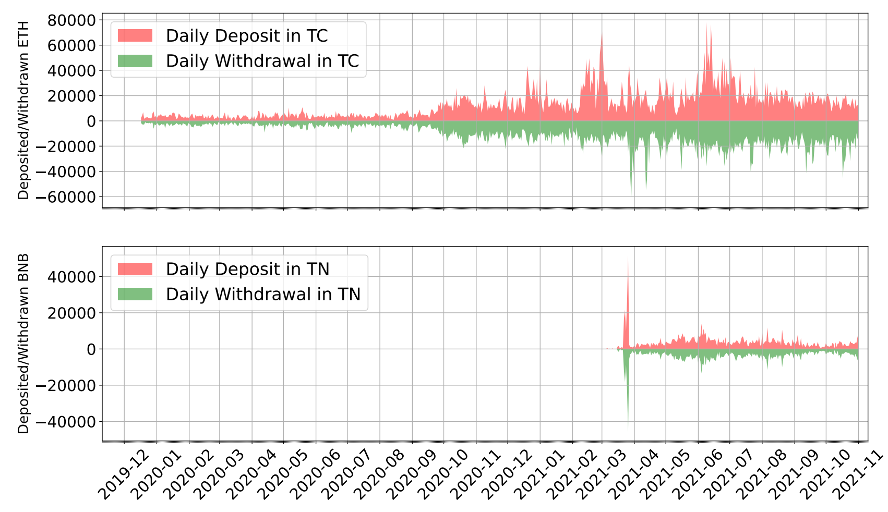
\includegraphics[width=0.5\textwidth]{tc.png} % Replace 'example-image' with the filename of your image
    \caption{Tornado Cash Interactions, \scriptsize{source: lecture 2}}
    \label{fig:image-example}
\end{figure}

\subsection{Security Implications of Censorship}
Assume a node is censoring transactions, now the questions is what does that node have to perform ? If a node doesn't just censor all of the incoming transactions, it has to go through a predefined list containing all the black-listed addresses. Thus it has to loop through this list and perform computations, check whether to censor it or not, hence has to use computational power on that transaction even though it will be drop at the end. Now an attacker could just generate a big batch of transactions an spam the node. For this transaction creation must be cheaper than transaction validation. The node then has to process this transactions and check if it should execute them. So we se that on the one hand censorship's is important to provide some legal compliance and fight against malicious users but on the other hand it is a platform for denial of service attacks and slows down transactions.
\\
\\
\textbf{Extra: Denial of Service Attacks:}\\
In this subsection we will quickly take a closer look at denial of service attacks on censoring nodes. We know that a Ethereum transaction involves different actors from validiators to miners etc. and each of those nodes can be responsible for censoring certain addresses. A DoS attack on those censoring nodes in a blockchain consist of flooding the network with transactions to overwhelm the nodes responsible for censoring transactions. So the nodes are occupied with other computations than censorship and thus leads to censorship policies getting ignored or increased  congestion in the system.

The following piece of code shows the structure of a computationally heavy transaction that could execute such a DoS attack:

\begin{figure}[h]
    \centering
    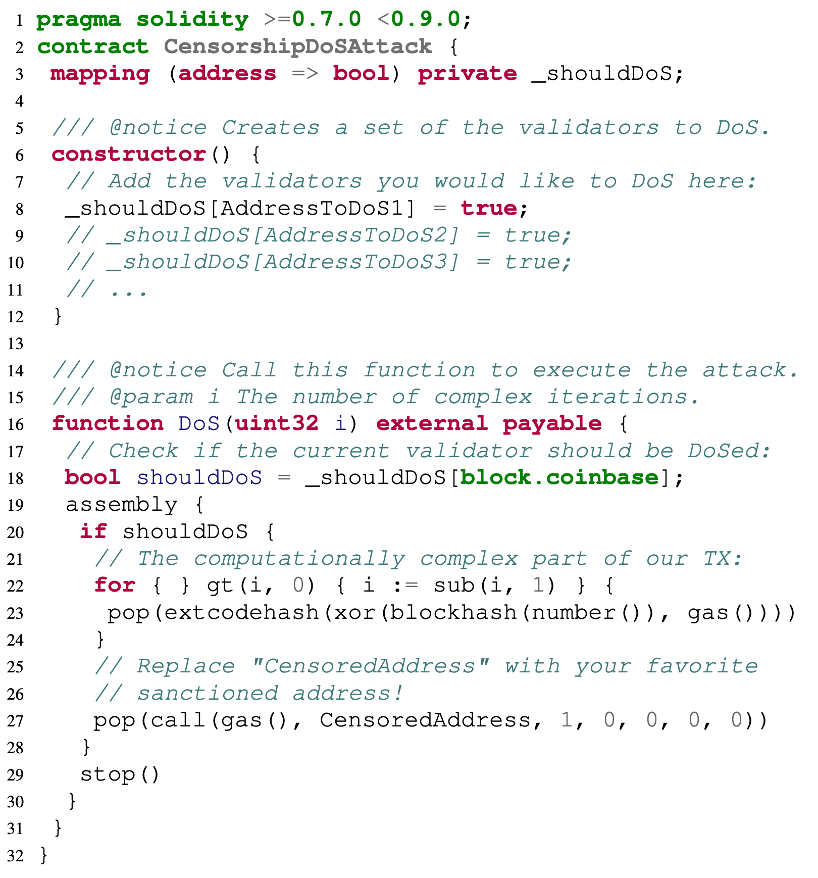
\includegraphics[width=0.5\textwidth]{dos-attack.png} % Replace 'example-image' with the filename of your image
    \caption{Example Code Of An Expensive Transaction, \scriptsize{source: lecture 2}}
    \label{fig:DoS-attack}
\end{figure}

\section{Quiz Content}
Here is a collection of terms, questions and topics covered in the lecture quizzes. I tried to structure them according to topic.

\begin{itemize}
    \item \textbf{Financial Inclusion}: Refers to accessibility and availability of financial services to actors, especially in under-served communities. All parts of society should have access to a range of affordable financial services like bank accounts, investment opportunities and credit services. Financial education is an additional important aspect of financial inclusion. 
    (taken from lecture slides)
    \item \textbf{Collateral}:  Assets that a borrower pledges to a lender to secure a loan.
    If the borrow can't repay the loan, the lender will become owner of the collateral to recover the outstanding debt.
    
    \item \textbf{Over-collateralization}: Refers to pledging more assets than required by the collateral requirements. If the requirements says 150\%, the borrower would have to provide collateral worth 150\% of the loan amount. Any collateral valued more than those 150\% would refer to over-collaterizing.\\
    Benefits of over-collaterization is
    \begin{itemize}
     \item {Risk reduction}:
        Having more collateral provides an extra protection for the lender, hence reduces his risk in case of loss.  
    \item {Market volatility protection}:
    As with over-collaterization the lender has more protection also against market volatility's. Stock prices and in general the value of assets fluctuates, with a over collaterized loan, the lender has a buffer against these ups and downs.
     \end{itemize}

     \item \textbf{Market Makers}: :
        Market makers are individuals or entities that are like the backbone of a market. They make it easier for people to trade, set prices, and keep things running smoothly. They constantly buy and sell stocks, bonds etc. to publicly stated prices and in that way ensure a liquid market. They kinda ensure that there is always a counter party if a trader wants to transact.
    \item \textbf{Bid-Ask-Spread}: Difference between the buying (bid) and the selling prices (ask). The goal is to buy at low prices and sell for a high prices. The difference is then called the spread and is a compensation for having provided liquidity to the market.
        
    \item \textbf{Transparency}: Transparency is a big keyword in DeFi. Technologies such as blockchain are transparent as they allow each user to see and trace every transaction. For some this transparent manner enhances trust for this financial system.
     \item \textbf{Financial Empowerment}: DeFi promises to empower the individuals by giving them more control and access over their assets. In DeFi the user often have a so called private key which allows them to directly engage in financial exchanges etc, without needing a traditional intermediaries.
      \item \textbf{Value at Risk aka "VaR"}: Is a statistical measure and describes the potential loss of an investment monitored over a time interval. VaR refer to an investment and a certain confidence level and estimate the maximum loss an investment is likely to incur with this confidence level.\\
For example, a 95\% VaR of \$1 million over one week means that there is a 95\% probability that the portfolio will not lose more than \$1 million over the next week.
\item \textbf{Excpected shortfall aka CVaR}:
Also known as Conditional Value at Risk (CVaR), is a risk measure that stands for the average loss that would occur beyond the VaR threshold. It represents the expected value of losses exceeding the VaR level.  
\item \textbf{ERC-20}: ERC20 is a token-management contract for Ethereum-based tokens. This means it's a set of rules and guidelines i.ex like an interface for tokens. The characteristics of such ERC-20 tokens are that they are fungible aka every token is identical to every other ERC-20 token, which is a useful characteristics in DeFi applications. This is of importance because they can be exchanged in a 1-to-1 ratio. ERC-20 has become the most used standard for tokens on the Ethereum blockchain.
(Btw ERC stands for "Ethereum Request For Comments and mirrors how protocols and standards are discussed and developed within the Ethereum community. Each users can review and take part in discussion about these suggested standards before they actually get implemented). 
\item \textbf{ERC-721}: As ERC-20 was a widely sued standart for fungiable tokens, ERC-721 is a standart typically used for Non-fungible tokens (NFTs) in Ethereum. It represents a set of rules and guidelines for representig ownership of NFT's. Each token created using the ERC-721 standard is distinct from every other token, hence they are non-fungible as each token has unique properties. This implies that they aren't exchanged on a 1-to-1 basis.

\item \textbf{Miners}: Mineras are essetial actors in the Ethereum network. They are responsible for including transactions into a block and creating new blocks. First Miners include pending transactions into blocks. Whenever a user wants to do a transaction (f. eg sending ETH to interact with a smart contract), it goes into the network and  miners will pick it up to process. The decision which miners can create the new block, the diffrent miners compete to solve a puzzle. This process is computationally intensive. When a miner has successfully solved the challenge he can create and provide the new block. For their efforts miners get newly created ETH (for each successfully mined block). Additionally they can also have to transaction fees within the block they mined.
\item \textbf{Transaction fees }:
 These are fees paid by users to miners to prioritize their transactions and ensure rapid of their transaction by miners.
\item \textbf{Block generation}: It describes the process of creating new blocks and adding them to the blockchain. It is done by the miners in a blockchain network. First there has to be a collection of transactions waiting be executed aka waiting to be in a block. Then the mining starts which means that miners compete in solving a puzzle, the first miner to solve it can create the new block and add it to the chain.
\\
\item \textbf{Anonymity Set}:Is the amount of deposits in a Tornado Cash pool. Refers to the level of privacy. F.eg a Tornado Cash pool with 1000 deposits has a anonymity set size of 1000 and a privacy level of 1/1000.


Liquiditiy Pools
LP Tokens ->can get her thigs out of the pool by provding the LP tokens (are usually fungiable)
\end{itemize}

\section{Decentralized Exchanges}
In this chapter we will look at so called DEX's, decentralized exchanges. In the finical world the exchanges are a center piece.There exist exchanges with all level of sophistication. A characteristic for a DEX is that it operates directly peer-to-peer without having a single trusted authority in the middle. But how do this exchanges operate ? How are the decentralized exchanges implemented ?

To make sure that we all are aware of why exchanges are useful and needed: Exchanges are platforms for individuals to buy, sell, and trade assets, in DEX's theses assets are mostly cryptocurrencies. In exchanges buyers and sellers get matched and overall exchanges make it easier for investors and companies to find a corresponding match.
\begin{figure}[h]
    \centering
    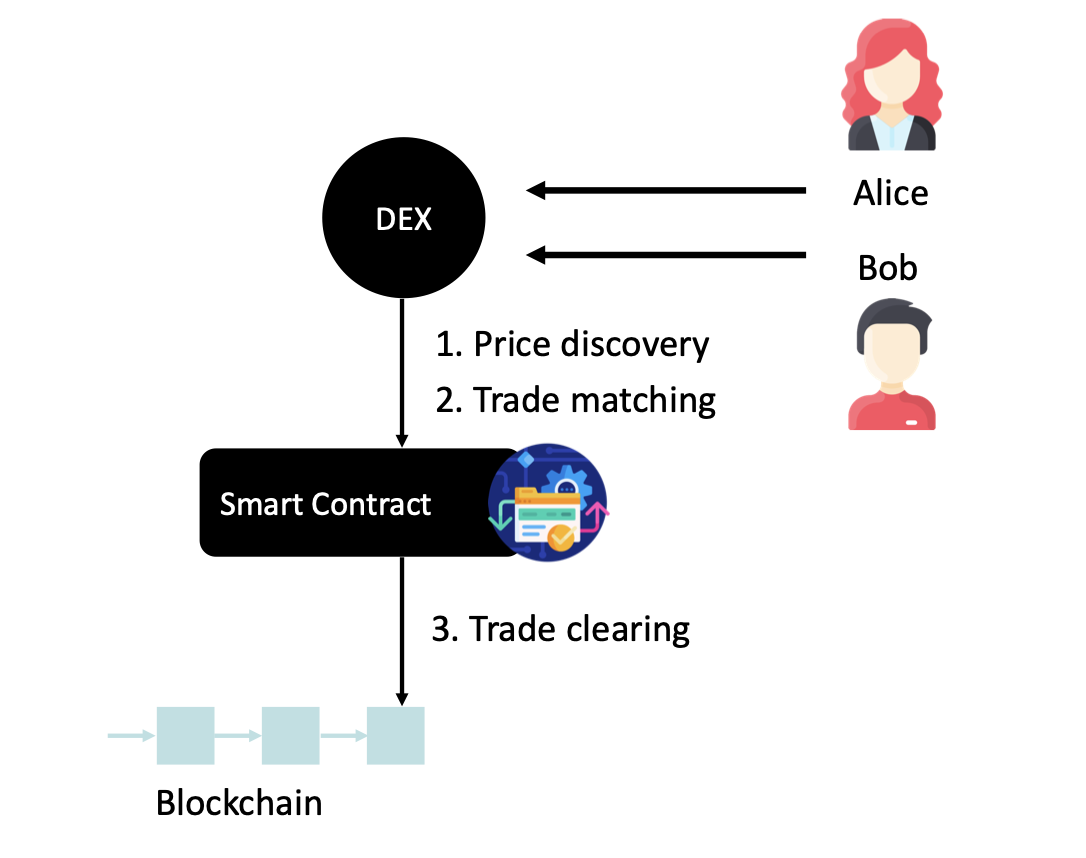
\includegraphics[width=0.5\textwidth]{Bildschirmfoto 2024-04-02 um 13.49.50.png} % Replace 'example-image' with the filename of your image
    \caption{Position of DEX, \scriptsize{source: lecture 4}}
    \label{fig:DoS-attack}
\end{figure}

What are steps that have to be done ?
\begin{itemize}
    \item {price discovery}
    \item {price matching}
    \item {actual transfer}
\end{itemize}


\subsection{Order books}
Order books are the core component of DeFi exchanges. They are an essential tool for traders to understand market liquidity and the amount of demand in the exchange. In Order book usually buy orders and sell orders are each listed on one side with corresponding information about the price and the quantity. The orders get placed by a so called market maker which gets to order request and puts them in them into the exchange system. An important characteristic of order books is the order depth. It stands for the level/amounts of buy and sell orders currently placed in the exchange and thus for the liquidity of the market. F.eg if the +2\% is CHF 2 million, the impact of a buy on the price is way less than when we have less depth f.eg if  the +2\% is only CHF 1000. So the order book depth is a signal of the price impact a buyer/seller will have and therefore a signal for the market liquidity. In order books there a two main types of orders a user can place:
\begin{itemize}
    \item {Market order}: As the name suggest it is an order where the users wants to buy or sell at the current market price. Thus these orders try to execute immediately at the currently best available price.
    \item {Limit Orders}: Limit orders try to buy or sell at a minimum/maximum of a specific price or better. If we issue a limit order, the order gets placed into the order book and will be realized if the market ever reaches the desired price level.\\
    \\
    Often an exchange is either a market order or a limited order book exchange. We refer to decentralized exchanges with limited order book mechanism as \textbf{LOB DEX's}.
\end{itemize}

\textbf{Advantages of LOB DEX'S}:
\begin{itemize}
    \item {No KYC/AML}: 
    \item {No fees for exchange}: 
    \item {No impermanent loss}: 
\end{itemize}
\textbf{Disadvantages}:
\begin{itemize}
    \item {Other fees }: 
    \item {Slow execution}: 
    \item {Not fully decentralized}:  
\end{itemize}
The last aspect of order books we will look at is the match making mechanism. Order books are like a matching engine that matches sellers and buyers with the best option for them in the order book. If there is no corresponding match, it just places it into the book and waits until it can be eventually executed at some future time point.

A keyword I want to mention here is the bit-ask spread. We will also see this definition in the "Quiz content chapter" but to summarize, the bit-ask spread describes how far away two participants aka a buyer and a seller are. The closer/ smaller the bit-ask spread, the more they match and to more satisfaction each actors gets from the exchange.\\
\\
Where does the order book run ? Earlier order books ran on a single server but as we can imagine running them on just a single server a lot can go wrong:A server can go down or become unavaible which would imply that the whole exchange is shut down and no one can trade. In addition single servers are vulnerable to flooing attacks where the server gets overwhelmed and disrupted, thus doesn't react anymore. And a key problem for DeFi is that a single server means we have to put trust into a single entity. That's exactly what decentralized strucutres tried to avoid and thus running order books on just a single server belongs to the past. Nowadays order books run on distributed system.

\section{Automated Market Maker}
An \textbf{automatic market maker (AMM)} is basically just a smart contract that does the market making in an autonomous way, hence doesn't need any third party to be involved. They are algorithms that automatically determine prices of assets etc. based on mathematical formulas which depend on the market liquidity. In AMM's users who want to do an exchange/trade provide liquidity into a so called liquidity pool. Each pool most ofen holds reserves for certain currencies and stands for a specific trading pair f.eg ETH to DAI and reverse. Then the AMM uses the lets call it "constanct product formula" to determine the price of a single investment in the pool. Hence when we as investors want to trade one currency for another we interact f.eg with an DeFi app which interacts with the corresponding liquidity pool. The AMM then calculates the price for the assets/trade based on the ratio or rather imbalance between the two currencies in the pool. So this means that the price of a of an assets in the pool changes depending on the trading activity.\\
\\
\begin{figure}[h]
    \centering
    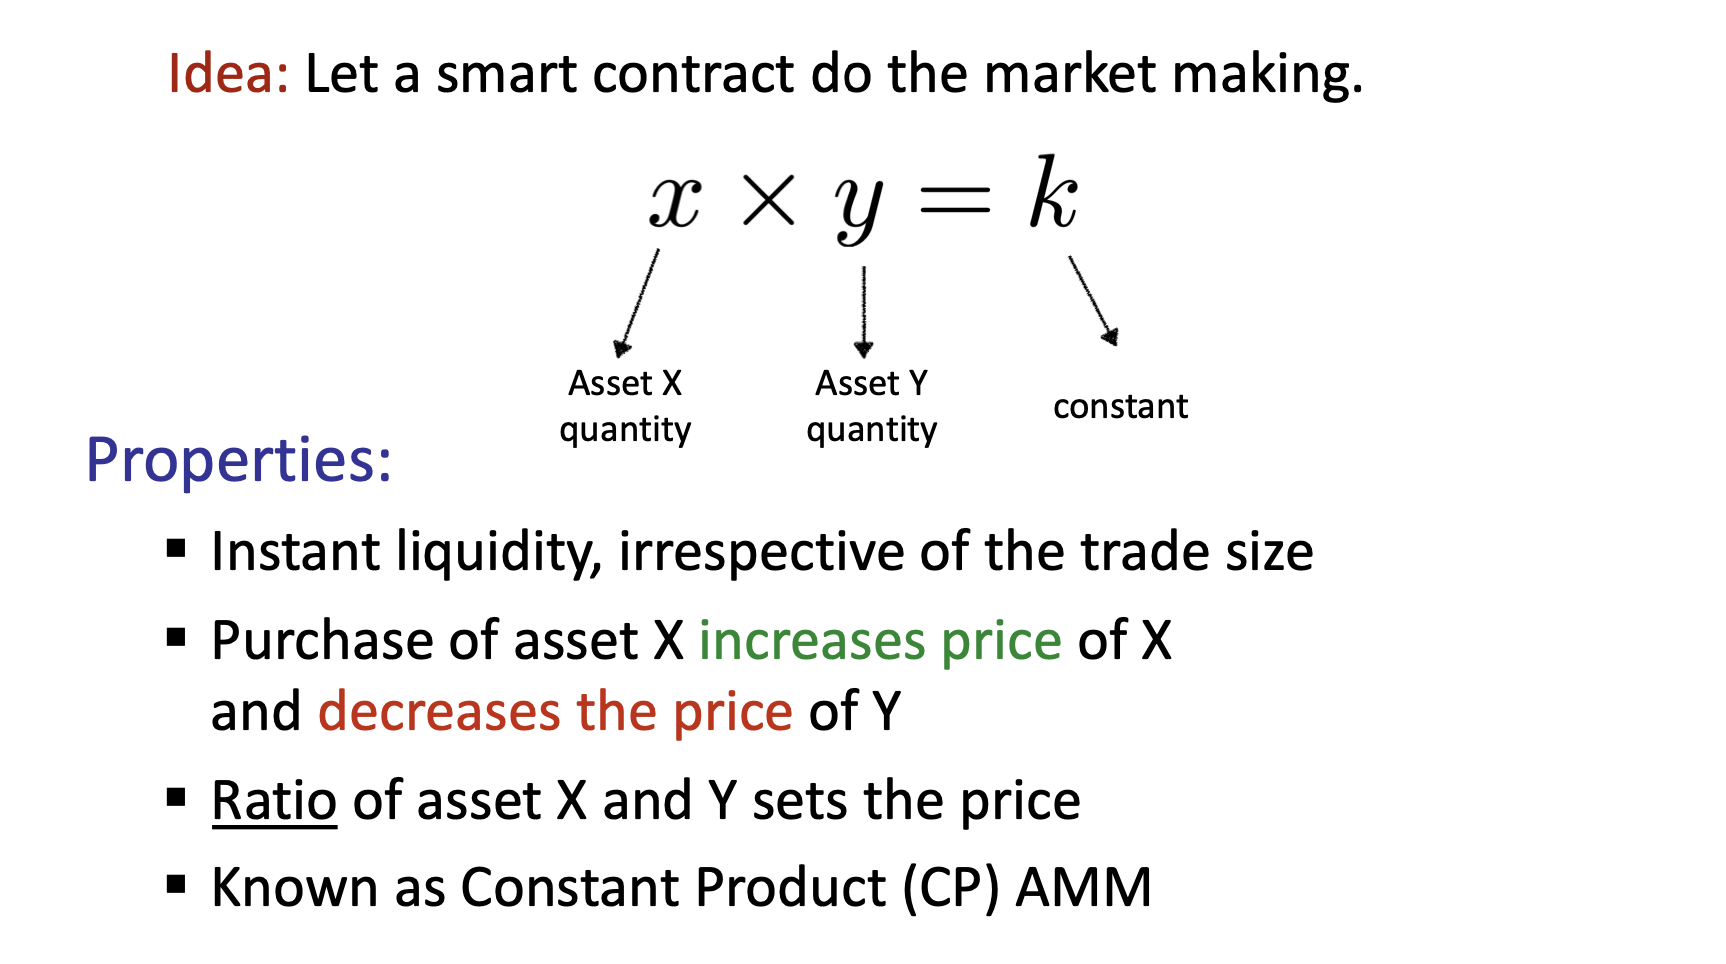
\includegraphics[width=0.5\textwidth]{Bildschirmfoto 2024-04-02 um 15.09.34.png} % Replace 'example-image' with the filename of your image
    \caption{Position of DEX, \scriptsize{source: lecture 4}}
    \label{fig:DoS-attack}
\end{figure}
\\

Pro: instant liqudity, don't have to wait for a MATCH, HERE ALWAYS HAVE A MATCH
downside of always matching: price changes, the more i want to buy the higher it is ->smoother than with order books. mORE SENSTIVE TO QUANTITY\\


AMM's are algorithms or one can also say protocols that allow decentralized exchanges to be simpler and (more) independent of third parties. Here I want to mention that there are multiple well know AMM's in the DeFi world like UniSwap or SushiSwap but even with AMM's we still have some centralized component as f.eg if users vote on important decision for such an AMM protocol there needs to be some organization that leads it. These organizations are so called decentralized autonomous organizations (DAOs). All we need to know is that they are responsible for holding votes about decisions for some DeFi protocols such as AMM's.\\
\\
To end this AMM chaptre we will walk throguh an example for a constant AMM. It should provide more understanding on how these proctols behave. I also want to mention that for AMMs the tokens involved in most cases are fungible, else defining a exchange ratio for this currencies is more complex. :\\
\begin{figure}[h]
    \centering
    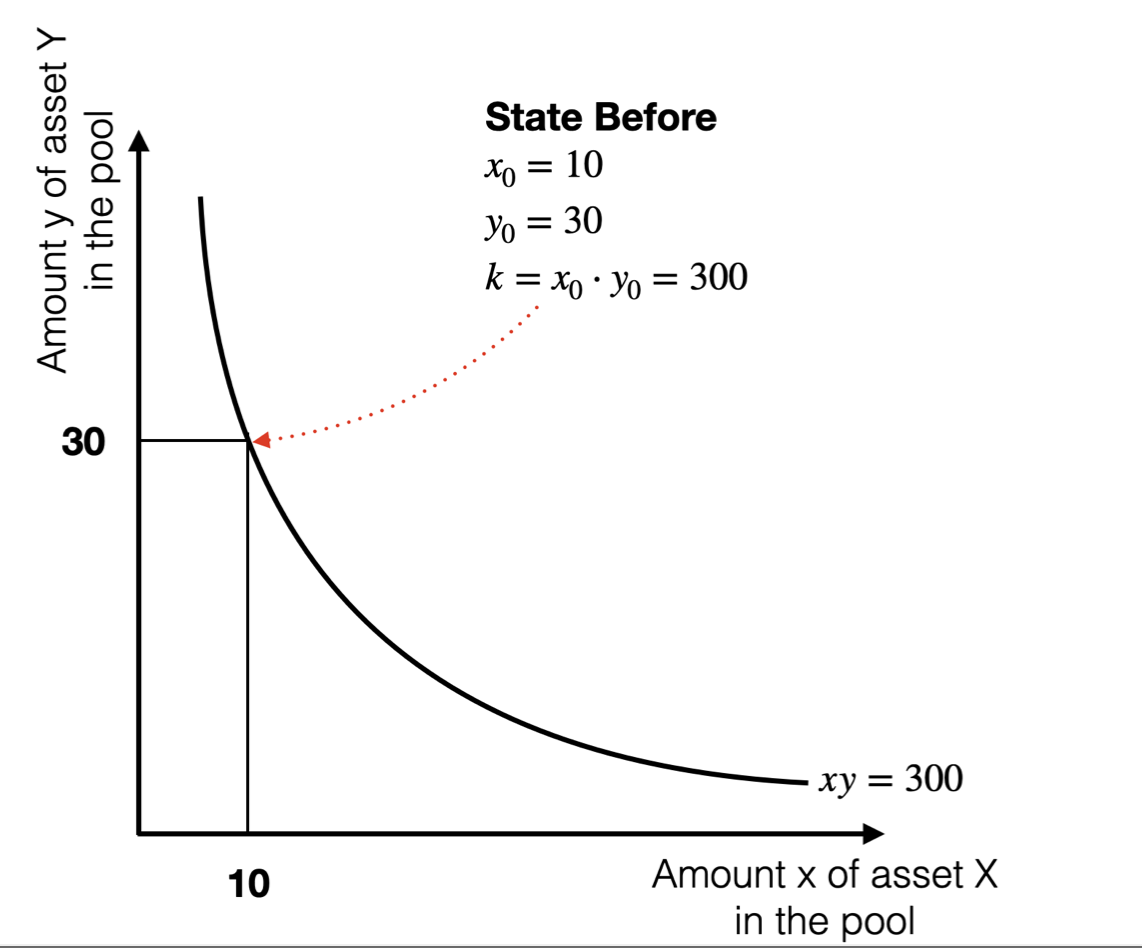
\includegraphics[width=0.5\textwidth]{Bildschirmfoto 2024-04-02 um 15.16.43.png} % Replace 'example-image' with the filename of your image
    \caption{Position of DEX, \scriptsize{source: lecture 4}}
    \label{fig:DoS-attack}
\end{figure}
\begin{itemize}
    \item {State before: In the pool are 10 assets of x and 30 assets of the currency y, now if we want to get 10 coins of the assets y, how many coins do we need to provide to the pool?}: 
    \item {As k needs to remain constant, we need to look at the equation and see how the parameters change. As we want to get 10 assets of y, the y amount will drop from 30 to 20 in the pool. Thus the x amount has to increase from 10 to 300/ 20 = 15. Hence we need to put 15-10 = 5 X coins into the pool.}:  
    \item {So if we provide at least 5 coins of X the smart contract is satisfied and we will get 10 coins of Y.}
\item {What happens if we add more liqudity to the pool, hence increase k ? In terms of prices nothing changes, only the constant product k is higher.}



\end{itemize}
What we observe with AMM's is the more we buy from an assets to more expensive each additional part gets. This phenomena is called the \textbf{expected slippage} and describes " the expected increase or decrease in price based on the trading volume and available liquidity" (quoted from lecture 4). The more liquidity of a certain coin we less impact a single trade of that coin has one the price. There is also the phenomena of \textbf{unexpected slippage}. This describe the price effect we get when we encounter an unexpected purchase of the same assets but that purchase is front running us, thus impacts our price execution. it can impact us in both directions, either we get a better or worse execution price. Now we may ask, can we then got a horrible price ? No, there is the possibility to fix a maximal slippage we are willing to accept. The transaction will fail if we cross the provided slippage limit

\subsection{Impermanent Loss} 
The effect/ loss we encounter through arbitrage. Called impermanent loss, because it is only a loss if we realize it aka withdraw from the pool. Else doesn't encounter the loss.
\textbf{Advantages of AMM}:
\begin{itemize}
    \item {no order book maintenance}
    \item {simple implementation}

\end{itemize}
\textbf{Disadvantages of AMM}:
\begin{itemize}
    \item {Danger of impermanent loss }: 
    \item {Slippage (especially in low liquidity markets}: 
    \item {sandwich attacks}:  
\end{itemize}






\section{DeFi Glossary}
\end{document}
